\chapter{Introduction\label{chap:intro}}

% Cold start
In this thesis, we develop an exact declarative programming based algorithmic approach for finding so-called Pareto-optimal solutions to bi-objective optimization problems encoded in propositional logic.

% What are optimization problems and where do they occur
% Start by telling a story (running example throughout intro)
Optimization problems can be summarized as the task of finding a ``best'' solution out of a collection of feasible ones.
For example, when looking for a new flat to buy, most people will be comparing prices with the aim to find the cheapest flat possible that fulfils their requirements.
Commonly, the notion of ``best'' that is used in optimization is that a solution with lowest associated ``cost'' is considered optimal.
In terms of the example above, cost is the price of a flat.
If the collection of possible solutions is discrete (as in this example), we speak of \emph{combinatorial} optimization.

% Real-world problems and hardness
For many real-world problems, the set of feasible solutions is too large to represent explicitly.
Instead, the feasible solutions are implicitly represented, often declaratively as a set of mathematical constraints.
Solving such an implicitly defined optimization problem is typically \NP-hard~\autocite{AroraBarak2009-complexity} and requires non-trivial algorithmic approaches.
Examples of such hard optimization problems appear in scheduling~\autocites{DBLP:conf/cp/Stojadinovic14,DBLP:conf/cpaior/BofillGSV15,DBLP:journals/ior/Solomon87,DBLP:journals/candie/AkyolB07}, supply chain optimization~\autocite{DBLP:journals/cce/Papageorgiou09}, air traffic management~\autocites{DBLP:journals/ior/BertsimasLO11,RichardsHow2002Aircrafttrajectoryplanning}, clustering~\autocite{DBLP:journals/ai/DaoDV17,DBLP:conf/sdm/DavidsonRS10}, optimal data representation~\autocites{DBLP:conf/cp/MaliotovM18,DBLP:conf/ijcai/NarodytskaIPM18,DBLP:conf/ijcai/Hu0HH20,DBLP:conf/cp/YuISB20,DBLP:conf/aaai/DemirovicS21,DBLP:conf/cp/ShatiCM21,DBLP:conf/cade/IgnatievPNM18}, among various other fields.

% Approaches to solving optimization
Different approaches to \NP-hard optimization have been proposed.
These approaches can be categorized as either exact or inexact.
Inexact approaches provide no guarantee of finding an optimal solution but return a \emph{good} solution within given resource constraints.
Examples of such approaches are local search~\autocite{DBLP:books/daglib/0017492} or evolutionary algorithms~\autocite{DBLP:books/daglib/0087893,DBLP:journals/jgo/StornP97}.
Exact approaches on the other hand are guaranteed to find an \emph{optimal} solution, given enough resources.
Central to exact approaches is the declarative approach to optimization.

% Solving pipeline for declarative approaches
The declarative approach to solving optimization problems, as shown in \cref{fig:solving-pipeline}, first encodes the original problem into a set of mathematical constraints formulated in an encoding language.
An encoding is hereby a mapping of each instance of the original problem to a set of constraints in the declarative language, where each optimal solution of the encoded instance corresponds to an optimal solution of the original instance.
Having encoded the problem instance, a so-called solver, an algorithm for finding optimal solutions for instances formulated in the encoding language, is invoked on the encoded instance to find a solution with the lowest cost.
As a last step, this found solution to the encoded instance is mapped back to the original problem space.

\begin{figure}
  \centering
  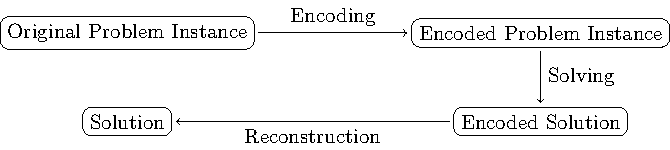
\includegraphics{solving-pipeline.pdf}
  \caption{The solving pipeline of the declarative approach to optimization.}\label{fig:solving-pipeline}
\end{figure}

% Advantages of the declarative approach and languages
An advantage of the declarative approach is that it is generally applicable to any problem, as long as a compact encoding for said problem exists.
When solving an optimization problem with the declarative approach, the challenge lies in choosing the encoding language that allows for a natural encoding and finding such an encoding.
Determining if a solution to constraints formulated in an encoding language exists is typically \NP-complete.
For a given declarative language, the existence of solvers that can \emph{efficiently} solve relevant optimization instances of said language is therefore critical as well.
Branch-and-cut algorithms for mixed integer linear programming (MILP)~\autocite{ChenEtAl2010-intro,KorteVygen2018-5} are an example of solver technology that achieves good performance on real-world instances.
The corresponding language of linear inequalities is arguably the most classical language for modelling hard optimization problems.
On the other hand, it might come as a surprise that the encoding language of propositional logic---which is very limited in expressiveness---has seen a stark increase in usage as well.
This is because recent research in propositional satisfiability (SAT)~\autocite{handbook2-sat} has seen much success using conflict-driven clause learning solvers~\autocite{handbook2-cdcl}.
This success has also been translated to optimization, in the form of maximum satisfiability (MaxSAT)~\autocite{handbook2-maxsat} solvers.

% Reveal conflicting second objective
It should be noticed that a clear majority of declarative optimization approaches, including MILP and MaxSAT, work under the assumptions that we are dealing with problems which intrinsically have a single objective to optimize.
However, this is not always the case.
Coming back to the flat search example, we notice that some requirements, like the number of rooms, might be easy to specify, but consider the distance of ones daily commute.
Rather than setting a fixed threshold such as ``maximum $d$ kilometres distance'', what we might actually want to do is minimize this distance at the same time as the cost of the flat.
Now there are two objectives to take into account regarding what constitutes a ``best'' solution.
Two or more objectives give rise to \emph{multi-objective} optimization.

% Conflicting objectives and why there might be no single optimal solution
A crucial difference between single- and multi-objective optimization is that there is no single notion of optimality for two or more objectives.
Whereas for a single objective function, there is a clear minimum (or maximum) and objective values can be unambiguously compared, this becomes less defined for the bi-objective case:
in the flat search example, consider a flat A with a cost of 300\,000 \texteuro{} and 1-kilometre daily commute and compare it to another flat B that costs 240\,000 \texteuro{} and has a 3-kilometre daily commute.
It is not immediately clear which one of these options is better, and the choice would depend on ones personal preference over the two objectives.
This becomes especially difficult if there is no such preference.
Typically, a situation like that occurs when two of the objectives considered are in conflict, as the price of a flat and the corresponding daily commute might be if the commute is towards the city centre and flats in the city centre are more expensive.

% Pareto optimality
% Point out different nomenclature
In this thesis, we use the commonly-used concept of \emph{Pareto optimality}%
\footnote{Pareto optimality is sometimes called \emph{efficiency}~\autocite{Ehrgott2005-2,DBLP:journals/siamjo/SantisENR20}}%
~\autocite{Ehrgott2005-2} as the notion of optimality.
Intuitively, under Pareto optimality a solution is considered optimal if no solutions that improve some objective without worsening the other exist.
As an example, this definition considers the two flats A and B from earlier both equally optimal.
Under Pareto optimality, the task of solving a bi-objective optimization problem exactly can mean multiple things:
finding a single Pareto-optimal solution, finding a representative solution for each Pareto point (i.e., tuple of Pareto-optimal objective values)%
\footnote{A Pareto point is also called a \emph{non-dominated point} in literature~\autocite{Ehrgott2005-2}}%
, or finding all Pareto-optimal solutions.
Most approaches~\autocite{DBLP:conf/cp/SohBTB17,DBLP:conf/cp/JanotaMSM21,DBLP:conf/ijcai/Terra-NevesLM18a} to solving multi-objective optimization under Pareto optimality appear to focus on the second task where a single solution per Pareto point is computed.
The last task goes one step further and enumerates the full Pareto front (i.e., all Pareto-optimal solutions), even if multiple of the solutions might lead to the same objective values.
All three of these tasks can be solved by the algorithmic approach presented in this thesis.

% Applications of bi-objective optimization in literature
The algorithmic approach presented in this thesis focuses on solving the common class of \emph{bi}-objective optimization problems, which have exactly two objective functions.
Bi-objective optimization problems arise naturally for various real-world settings.
For example, when learning interpretable classifiers~\autocites{DBLP:conf/ijcai/Ignatiev0NS21,DBLP:conf/cp/MaliotovM18,DBLP:conf/ijcai/NarodytskaIPM18,DBLP:conf/ijcai/Hu0HH20,DBLP:journals/corr/abs-2010-09919,DBLP:conf/cp/YuISB20,DBLP:conf/aaai/Ignatiev0S021,DBLP:conf/cade/IgnatievPNM18}, the objectives ``interpretability'' and ``classification error'' are in conflict because a more complex and therefore less interpretable classifier is typically more accurate.
As another example, a bi-objective optimization problem arises when wanting to create a portfolio of solvers that together solve a set of benchmarks as fast as possible while also containing as few solvers as possible~\autocite{DBLP:conf/cp/JanotaMSM21}.
There are also bi-objective optimization problems in network routing with the objectives load balancing and latency~\autocite{SilverioEtAl2022biobjectiveoptimization}.
In supply chain optimization, in addition to the economic objective, environmental aspects can be taken into consideration as a second objective~\autocites{DBLP:journals/cce/Pinto-VarelaBN11,DBLP:journals/candie/TautenhainBN19}.

% Contributions
% Algorithm: single SAT solver; builds on MaxSAT; single vs all
The main contribution of this work is the \algname{} algorithm, a MaxSAT-based bi-objective optimization approach.
\algname{} follows the lexicographic method~\autocite{survey}, which works by minimizing the objective which we call increasing first and afterwards minimizing the decreasing objective under the constraint that the increasing one cannot get worse.
Once the first Pareto point has been found, the search continues by minimizing the increasing objective again, but under the constraint that the decreasing objective should be smaller than before.
Note the difference between this lexicographic \emph{method} compared to lexicographic \emph{optimization}~\autocite{DBLP:conf/ijcai/ArgelichLS09,DBLP:journals/amai/Marques-SilvaAGL11} to which SAT-based approaches have been proposed earlier.
Lexicographic optimization only considers the first Pareto point, found by the lexicographic method, optimal.

% Variants
\algname{} builds on advances in MaxSAT solving, allowing for variants based on different solution-improving~\autocites{handbook2-maxsat,DBLP:journals/jsat/BerreP10,DBLP:journals/jsat/EenS06} and core-guided~\autocites{DBLP:journals/corr/abs-0712-1097,DBLP:conf/sat/AnsoteguiBL09,DBLP:conf/cp/MorgadoDM14,DBLP:journals/jsat/IgnatievMM19} algorithms.
We propose five different variants of \algname{} that differ in how the minimization of the increasing objective is done.
The first four building on the SAT-UNSAT~\autocite{DBLP:journals/jsat/BerreP10}, UNSAT-SAT~\autocite{DBLP:conf/sat/FuM06}, MSU3~\autocite{DBLP:journals/corr/abs-0712-1097} and OLL~\autocite{DBLP:conf/cp/MorgadoDM14} MaxSAT algorithms, modifying them mainly in the fact that a bound on the decreasing objective needs be enforced during optimization.
The fifth variant is a hybrid switching from the MSU3- to the SAT-UNSAT-based variant during the search, aiming to combine the advantages of the two approaches.
In addition to five variants of \algname{}, we also propose multiple refinements for improving its performance:
lazily building the cardinality constraints for both objectives to reduce the number of clauses in the solver, blocking dominated solutions to prune the search space, more efficient domain-specific blocking clauses, bound hardening to enable the solver to learn more information and other refinements known from core-guided MaxSAT solving.
\algname{} allows for solving all three tasks for bi-objective optimization:
finding a single Pareto-optimal solution, one representative solution for each Pareto point or enumerating all Pareto-optimal solutions.

% Evaluation: study efficiency of different MaxSAT algorithms
We provide an open-source implementation of all five variants of \algname{} ({\small\url{https://bitbucket.org/coreo-group/bioptsat/}}) and empirically evaluate its performance on two benchmark domains:
learning interpretable decision rules from binary data~\autocite{DBLP:conf/cp/MaliotovM18} (as a generalization of settings for which MaxSAT-based single-objective solutions have been previously proposed) and bi-objective set covering.
In the experiments, we compare \algname{} to three key SAT-based competitors:
enumeration of so-called $P$-minimal solutions~\autocite{DBLP:conf/cp/SohBTB17}, ParetoMCS enumeration~\autocite{DBLP:conf/ijcai/Terra-NevesLM18a} and Seesaw~\autocite{DBLP:conf/cp/JanotaMSM21}.
We find that \algname{} outperformed these competitors in all studied cases.
As an additional result of this evaluation, we determine which variant of \algname{} is the best-performing overall.
Furthermore, for the best-performing variant, we study the effects of the proposed refinements to determine their effectiveness.

% Signposting for chapters
This thesis is structured as follows.
An overview of propositional satisfiability and maximum satisfiability, highlighting the important preliminaries needed to understand the proposed algorithm, is given in \cref{chap:satisfiability}.
In \cref{chap:biobjective-optimization}, we introduce bi-objective optimization, defining the problem and surveying key existing algorithmic approaches to bi-objective optimization.
After that, in \cref{chap:approach}, we describe \algname{}, including five distinct variants and some refinements.
Details on the empirical evaluation of our implementation are provided in \cref{chap:experiments}.

% Acknowledging the paper
Results presented in this thesis have been published in the proceedings of the 25th International Conference on Theory and Applications of Satisfiability Testing (SAT 2022)~\autocite{JabsEtAl2022MaxSATBasedBi}.
In this thesis, we extend on the empirical evaluation and give a more in-depth description of the preliminaries and the algorithm itself, compared to~\autocite{JabsEtAl2022MaxSATBasedBi}.